\documentclass[11pt]{article}
\usepackage{amsmath}
\usepackage{graphicx}
\graphicspath{{img/}}

\begin{document}

\title{{\bf 11-755: MLSP}\\
       HW \#3: Clustering and EM}

\author{Nikolas Wolfe}

\date{December 15, 2015}
\maketitle


\section*{Problem 1: K-Means \& Spectral Clustering}
You are given a number of toy datasets. The visulized groud truth clustering configuration of these data: Aggregation (K=7), Bridge (K=2), Compound (K=6), Flame (K=2), Jain (K=2), Spiral (K=3) and TwoDiamond (K=2) are shown as follows:
\begin{center}
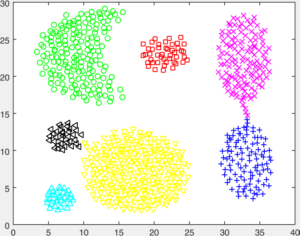
\includegraphics[scale=0.5]{aggregation}
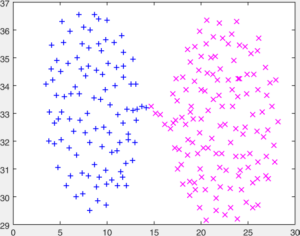
\includegraphics[scale=0.5]{bridge}
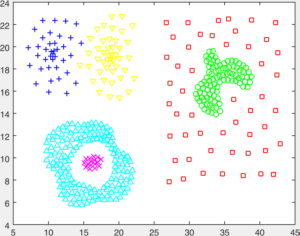
\includegraphics[scale=0.5]{compound}
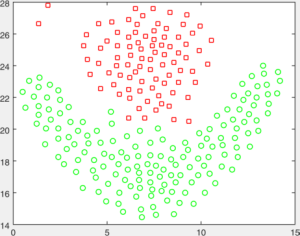
\includegraphics[scale=0.5]{flame}
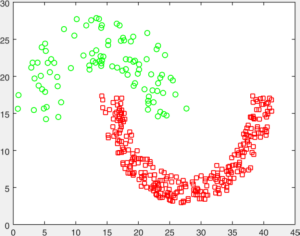
\includegraphics[scale=0.5]{jain}
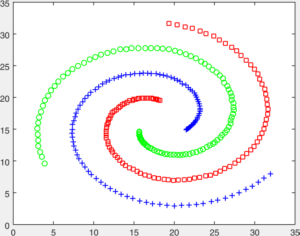
\includegraphics[scale=0.5]{spiral}
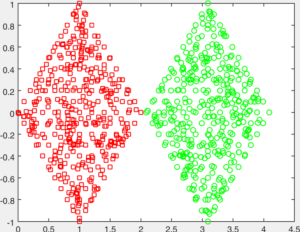
\includegraphics[scale=0.5]{twoDiamonds}
\end{center}
{\bf Answer:} 
I implemented this code in Java, using the Efficient Java Matrix Library (EJML) package to do matrix multiplication and Eigen/Singular Value decomposition. In order to 

\pagebreak
\section*{Problem 2: Expectation Maximization}

\end{document}